% !TEX TS-program = xelatex
% !TEX program = xelatex
% !TEX encoding = UTF-8 Unicode

\documentclass[12pt]{article}

\usepackage{fontspec}
\usepackage{ifxetex}
\usepackage[margin=1in]{geometry}
\usepackage{enumitem}
\usepackage{setspace}
\usepackage{fancyhdr}
\usepackage{graphicx}
\usepackage{hyperref}
\usepackage{longtable}
\usepackage{booktabs}
\usepackage{caption}
\usepackage{array}
\usepackage{calc}
\makeatletter
\@ifundefined{ul}{\newcommand{\ul}{\underline}}{}
\@ifundefined{none}{\newcounter{none}}{}
\makeatother

\setstretch{1.15}

% Thai font settings (XeLaTeX)
\IfFontExistsTF{Laksaman}{
  \setsansfont{Laksaman}[
    BoldFont       = Laksaman Bold,
    ItalicFont     = Laksaman Italic,
    BoldItalicFont = Laksaman Bold Italic
  ]
  \setmainfont{Laksaman}[
    BoldFont       = Laksaman Bold,
    ItalicFont     = Laksaman Italic,
    BoldItalicFont = Laksaman Bold Italic
  ]
}{
  \setsansfont[
    Path           = ./fonts/,
    UprightFont    = Laksaman.ttf,
    BoldFont       = Laksaman-Bold.ttf,
    ItalicFont     = Laksaman-Italic.ttf,
    BoldItalicFont = Laksaman-BoldItalic.ttf
  ]{Laksaman.ttf}
  \setmainfont[
    Path           = ./fonts/,
    UprightFont    = Laksaman.ttf,
    BoldFont       = Laksaman-Bold.ttf,
    ItalicFont     = Laksaman-Italic.ttf,
    BoldItalicFont = Laksaman-BoldItalic.ttf
  ]{Laksaman.ttf}
}

% Thai line breaking (XeLaTeX only)
\ifxetex
  \XeTeXlinebreaklocale "th"
  \XeTeXlinebreakskip = 0pt plus 1pt
\fi

\providecommand{\tightlist}{%
  \setlength{\itemsep}{0pt}\setlength{\parskip}{0pt}}

% ========== HEADER & FOOTER ============
\pagestyle{fancy}
\fancyhf{}
\fancyfoot[R]{\thepage}
\renewcommand{\headrulewidth}{0pt}

\begin{document}
\textbf{Computer Engineering Capstone Project Proposal I}

\textbf{Project AiQ}

Intelligence That Drives Execution

An AI-driven Knowledge Management Platform

\textbf{Team}

\begin{quote}
Chawin Leardswai 6633047821

Tanit Yodsirawong 6633104921

Nattapol Teerayuttawong 6633072421

Peerapat Patcharamontree 6633176021

Puran Prasertthai 6633154221
\end{quote}

\textbf{Advisor}

\begin{quote}
Chulalongkorn University

Asst. Prof. Sukree Sinthupinyo, Ph.D.

Assoc. Prof. Twittie Senivongse, Ph.D.

SCB TECH X CO., LTD.

Chanintorn Asavavichairoj\\
Jessada Weeradetkumpon
\end{quote}

\section{\texorpdfstring{\hfill\break
}{ }}\label{section}

\section{Abstract}\label{abstract}

This project, Project AiQ - "Intelligence That Drives Execution",
addresses the critical problem of fragmented enterprise knowledge
scattered across systems like SharePoint, by designing a secure and
scalable AI-driven Knowledge Hub to automate retrieval and improve
organizational efficiency.

To achieve this, the proposed solution involves designing and
implementing a Retrieval-Augmented Generation (RAG) system, specifically
focusing on a scalable data ingestion and preparation pipeline that
utilizes GraphRAG techniques to securely structure content from
enterprise sources.

The expected outcomes include a detailed technical design, an
implemented data pipeline with foundational Single Sign-On (SSO)
security, a minimal RAG Web Chat MVP, and significant contributions to
both academic validation of the RAG architecture and industrial benefits
through improved efficiency and knowledge consolidation.

\textbf{Keywords:} RAG, Knowledge Management, Data Ingestion, Enterprise
AI, GraphRAG

\section{Table of Contents}\label{table-of-contents}

\hyperref[abstract]{\textbf{Abstract 1}}

\hyperref[table-of-contents]{\textbf{Table of Contents 2}}

\hyperref[introduction-problem-definition]{\textbf{1. Introduction \&
Problem Definition 3}}

\begin{quote}
\hyperref[background-motivation]{1.1 Background \& Motivation 3}

\hyperref[problem-statement]{1.2 Problem Statement 3}

\hyperref[objectives]{1.3 Objectives 3}

\hyperref[scope-limitations]{1.4 Scope \& Limitations 4}

\hyperref[expected-benefits]{1.5 Expected Benefits 4}
\end{quote}

\hyperref[problem-solving-related-work]{\textbf{2. Problem Solving \&
Related Work 5}}

\begin{quote}
\hyperref[review-of-existing-knowledge]{2.1 Review of Existing Knowledge
5}

\hyperref[comparison-with-existing-systems]{2.2 Comparison with Existing
Systems 6}

\hyperref[gap-analysis]{2.3 Gap Analysis 6}

\hyperref[linkage-to-project]{2.4 Linkage to Project 7}
\end{quote}

\hyperref[proposed-solution-design-concept]{\textbf{3. Proposed Solution
/ Design Concept 8}}

\begin{quote}
\hyperref[system-overview]{3.1 System Overview 8}

\hyperref[components]{3.2 Components 8}

\hyperref[diagrams]{3.4 Diagrams 11}
\end{quote}

\hyperref[teamwork-plan]{\textbf{4. Teamwork Plan 14}}

\begin{quote}
\hyperref[roles-and-responsibilities]{4.1 Roles and Responsibilities 14}

\hyperref[collaborative-plan]{4.2 Collaborative Plan 14}

\hyperref[task-coverage]{4.3 Task Coverage 14}

\hyperref[workload-balance]{4.4 Workload Balance 14}
\end{quote}

\hyperref[timeline]{\textbf{5. Timeline 14}}

\hyperref[semester-1]{\textbf{Semester 1 14}}

\hyperref[semester-2]{\textbf{Semester 2 15}}

\textbf{6\hyperref[ethics-privacy-and-professional-considerations]{.
Ethics, Privacy, and Professional Considerations 16}}

\begin{quote}
6\hyperref[credibility-of-information]{.1 Credibility of Information 16}
\end{quote}

\hyperref[references]{\textbf{References 17}}

\hyperref[appendices]{\textbf{Appendices 18}}

\begin{quote}
\hyperref[wireframes-and-mockups]{Wireframes and Mockups 18}

\hyperref[early-test-datasets]{Early Test Datasets 19}
\end{quote}

\section{\texorpdfstring{\hfill\break
}{ }}\label{section-1}

\section{1. Introduction \& Problem
Definition}\label{introduction-problem-definition}

\subsection{1.1 Background \& Motivation}\label{background-motivation}

Modern enterprise environments, including organizations that manage
large and complex projects like \textbf{SCB TechX}, often face a common
problem: important project information is \textbf{scattered across many
different systems}. Emails, shared file drives, and internal tools such
as SharePoint all contain pieces of knowledge, but none of them provide
a complete picture. As a result, finding the right information becomes
slow, inconvenient, and sometimes confusing.

To solve this, organizations are moving toward a \textbf{Knowledge Hub}
concept, which requires a system that not only consolidates data but
also provides intelligent access. The central challenge, which motivates
this research-focused project, is the initial step: how to securely and
efficiently ingest this fragmented data and transform it into a unified,
queryable knowledge base. By creating a robust ingestion and preparation
pipeline early on, we aim to lay the groundwork for using AI to automate
knowledge retrieval, thereby addressing inefficiency issues and ensuring
project continuity.

\subsection{1.2 Problem Statement}\label{problem-statement}

The core engineering problem is to design, research, and validate the
technical foundation for a secure and scalable AI-driven knowledge
management platform. Specifically, the problem centers on:

\begin{enumerate}
\def\labelenumi{\arabic{enumi}.}
\item
  Designing a robust content extraction and preparation pipeline that
  can handle data from enterprise-level sources (e.g., SharePoint) and
  structure it for semantic search.
\item
  Formulating a security strategy that integrates with existing
  enterprise authentication methods, such as SSO (Single Sign-On).
\item
  Integrating the AI and Distributed Systems disciplines to ensure the
  initial data ingestion architecture is scalable and reliable, which is
  a complex requirement for real-world enterprise deployment.
\end{enumerate}

This research and design effort is complex and meaningful because
successfully managing the "first mile" of data ingestion and preparation
dictates the accuracy and performance of the subsequent RAG pipeline, a
non-trivial challenge that requires creative integration of various
computer engineering sub-disciplines.

\subsection{1.3 Objectives}\label{objectives}

The project aims to achieve the following clear, measurable goals in a
phased, two-semester approach:

\begin{enumerate}
\def\labelenumi{\arabic{enumi}.}
\item
  Research and Design (Capstone I Focus): Conduct comprehensive research
  on current RAG architectures, perform a gap analysis of existing
  knowledge management systems, and deliver a detailed technical design
  for the entire system, emphasizing the data ingestion and content
  extraction pipeline.
\item
  Data Preparation Pipeline Development (Implementation Focus): Design
  and implement a scalable data ingestion and preparation pipeline
  capable of securely connecting to and extracting content from a
  primary enterprise source (e.g., SharePoint).
\item
  Foundational Integration (Implementation Focus): Implement the
  foundational security integration to support Single Sign-On (SSO),
  ensuring secure user access to the system.
\item
  Evaluation: Define key performance metrics for the data pipeline
  (e.g., latency, throughput) and the RAG model\textquotesingle s
  accuracy, with testing to commence in Capstone II.
\end{enumerate}

\subsection{1.4 Scope \& Limitations}\label{scope-limitations}

Scope

\begin{enumerate}
\def\labelenumi{\arabic{enumi}.}
\item
  Research \& Proposal (Capstone I): Deliver a full written proposal and
  research review.
\item
  Data Ingestion \& Preparation: Design and implement the ingestion of
  unstructured and semi-structured data from SharePoint and a general
  file upload feature. This includes content extraction, chunking, and
  embedding.
\item
  Security Foundation: Implement Single Sign-On (SSO) for secure user
  authentication.
\item
  Interface: Develop a minimal Web Chat MVP with basic prompt and
  response functionality to demonstrate RAG output.
\end{enumerate}

Limitations

\begin{enumerate}
\def\labelenumi{\arabic{enumi}.}
\item
  Initial data ingestion implementation will focus on one primary
  enterprise source (Xhive).
\item
  Advanced access control mechanisms (e.g., RBAC ) are considered
  complex and will be scaled back to basic authentication checks (SSO)
  as advanced access control is considered a future enhancement.
\item
  Advanced user-facing features (e.g., multi-channel integration via
  LINE/MS Teams) are out-of-scope for the MVP and reserved for future
  work.
\end{enumerate}

\subsection{1.5 Expected Benefits}\label{expected-benefits}

The project is structured to maximize academic and professional impact

\textbf{Academic/Technical Benefit:}

\begin{enumerate}
\def\labelenumi{\arabic{enumi}.}
\item
  Validated Architecture: Deliver a thoroughly researched and documented
  architecture for a complex enterprise RAG system.
\item
  Data Pipeline Expertise: Provide practical experience in designing and
  implementing a robust data ingestion pipeline that handles real-world,
  messy, and large-scale organizational data.
\item
  RAG Optimization: Provide a testbed for evaluating the performance
  implications of different RAG components (e.g., chunking strategies,
  re-ranking).
\end{enumerate}

\textbf{Industrial/Professional Benefit:}

\begin{enumerate}
\def\labelenumi{\arabic{enumi}.}
\item
  Efficiency: Lay the foundation to reduce the time spent searching for
  information, leading to eventual cost savings and improved team
  agility.
\item
  Knowledge Consolidation: Create a centralized platform that turns
  scattered documentation into an accessible Knowledge Hub.
\item
  Streamlined Onboarding: Improve the onboarding process for new joiners
  by providing an immediate, centralized, and intelligent way to access
  project history and essential internal knowledge.
\end{enumerate}

\section{2. Problem Solving \& Related
Work}\label{problem-solving-related-work}

\subsection{2.1 Review of Existing
Knowledge}\label{review-of-existing-knowledge}

In large-scale enterprise environments, knowledge is generally locked
within different repositories, such as emails, cloud drives, or
collaboration platforms, which makes the extraction of information less
efficient. The traditional approach to Knowledge Management is based on
keyword indexing, such as Inverted Indices, which fail to capture the
semantic intent of user queries or contextual relationships between
documents {[}1{]}.

To overcome these limitations, Retrieval-Augmented Generation (RAG) has
emerged as a standard architecture. RAG enhances Large Language Models
(LLMs) by retrieving relevant data from a private knowledge base (the
Vector Store) before generating an answer {[}2{]}. The RAG mechanism
involves key steps: query transformation, retrieval (using a Vector
Store based on semantic similarity), and the final generation step.
However, the efficacy of a RAG system is strictly dependent on robust
data management strategies, such as text chunking and document ranking
{[}3{]}.

Current academic and industrial research indicates that standard
"out-of-the-box" ingestion pipelines often perform naive text chunking
(e.g., fixed window size). They slice documents arbitrarily, severing
the logical flow and losing critical metadata (such as file hierarchy or
authorship). To build a robust Knowledge Hub, modern approaches must
utilize High-Fidelity Ingestion Pipelines. These pipelines combine
Vector Embeddings (to capture semantic meaning) with Graph/Relational
Structures (a technique known as GraphRAG, to map explicit relationships
between entities and documents), ensuring that the data fed into the AI
is clean, structured, and context-aware. This project emphasizes
researching and implementing advanced techniques, including recursive
text splitting and Graph-based chunking, to maximize context
preservation. {[}4{]}.

\subsection{2.2 Comparison with Existing
Systems}\label{comparison-with-existing-systems}

The existing solutions of enterprise knowledge retrieval could be
grouped into three levels of maturity.

\textbf{Level 1: Legacy Keyword Search (e.g., Standard Repository
Search)}

\begin{itemize}
\item
  \textbf{Mechanism}: Matches exact keywords in file names or contents.
\item
  \textbf{Weakness}: Returns lists of files rather than answers. It
  cannot handle synonyms or natural language questions
\item
  \textbf{Relevance}: Serves as the baseline that this project aims to
  surpass.
\end{itemize}

\textbf{Level 2: Naive/Generic RAG Implementations}

\begin{itemize}
\item
  \textbf{Mechanism}: Ingests text directly into a vector store using
  fixed-window chunking (e.g., every 500 tokens).
\item
  \textbf{Weakness}: Suffers from Context Fragmentation. Since text
  chunking often disregards the logical structure, the relationship
  between topics and content is lost. This prevents the model from
  correctly linking information and often leads to "hallucinations"
  (generating false information) due to the lack of structural integrity
  in the input data {[}5{]}.
\item
  \textbf{Relevance}: Reflects a critical limitation that this project
  aims to address by prioritizing the engineering foundation from the
  very first step (The First Mile of Engineering).
\end{itemize}

\textbf{Level 3: The Proposed Pipeline-Centric System
(GraphRAG-enhanced)}

\begin{itemize}
\item
  \textbf{Mechanism}: Prioritizes the Data Ingestion Layer. It employs a
  custom extraction pipeline (utilizing tools like the Docling framework
  {[}6{]} or similar advanced parsers) that rigorously sanitizes data,
  preserves document hierarchy, and constructs a hybrid knowledge
  representation. This representation combines semantic vectors (in
  Qdrant) with explicit relational context (in a separate Graph Store
  like Neo4j, or through metadata filtering) before the data reaches the
  AI model.
\item
  \textbf{Strength}: Ensures high-fidelity input for the RAG model,
  significantly reducing hallucinations and improving the
  system\textquotesingle s ability to handle complex, context-dependent
  queries.
\end{itemize}

\subsection{2.3 Gap Analysis}\label{gap-analysis}

Despite the many existing RAG frameworks and tools, there are
considerable limitations to applying them in an enterprise context such
as SCB TechX:

\begin{itemize}
\item
  \textbf{Limitation regarding Data Ingestion (The Ingestion Gap)}: Most
  open-source tools focus on the retrieval algorithm (the AI side) but
  neglect the ingestion complexity (the Data Ingestion side). There is a
  lack of robust pipelines designed to handle "messy" enterprise data
  formats while preserving semantic structure. Solving this requires
  specialized document parsing and OCR tools to extract high-fidelity
  content.
\item
  \textbf{Limitation regarding Data Synchronization (The Synchronization
  Gap)}: Standard RAG implementations often treat knowledge bases as
  static datasets that require manual re-indexing. In active enterprise
  environments, data evolves constantly. There is a critical shortage of
  systems capable of Real-time Synchronization, where updates in the
  source (e.g., SharePoint) are instantly reflected in the
  AI\textquotesingle s knowledge base without downtime. This requires a
  dedicated event-driven architecture using services like a Webhook
  Listener and a Message Queue (RabbitMQ).
\item
  \textbf{Limitation regarding Context (The Contextual Gap)}: Standard
  vector search flattens data, losing the "relational" context (e.g.,
  distinguishing between a draft and a final policy, or linking a
  meeting minute to its specific project). Current systems rarely
  combine vector search with relational filtering effectively. This gap
  requires implementing GraphRAG-style extraction to create a structured
  knowledge graph that preserves relationships between content chunks
  and documents.
\end{itemize}

\subsection{2.4 Linkage to Project}\label{linkage-to-project}

This project addresses the identified limitations by focusing heavily on
the Ingestion and Preparation Pipeline:

\begin{enumerate}
\def\labelenumi{\arabic{enumi}.}
\item
  \textbf{Optimized Data Ingestion}: By designing a robust content
  extraction system, the project ensures that unstructured data from
  sources like Xhive/SharePoint is transformed into high-quality,
  queryable assets. This directly solves the "Ingestion Gap."
\item
  \textbf{Automated Knowledge Synchronization}: The project implements
  an automated pipeline that monitors source repositories for changes.
  This bridges the "Synchronization Gap" by ensuring that when files are
  added or modified in SharePoint, the AI's knowledge base is updated in
  near real-time without manual re-indexing.
\item
  \textbf{Hybrid Data Representation}: By researching and implementing a
  system that understands both the content and the structure/metadata of
  the files, the project addresses the "Contextual Gap," creating a
  semantic space that allows the AI to retrieve information with higher
  precision than standard flat searches.
\end{enumerate}

To implement these solutions, the project takes a deep dive into the
technical implementation of specific tools, including CrewAI for
multi-agent reasoning, Qdrant for vector operations and relational
filtering, and custom ETL pipelines utilizing advanced libraries for
semantic and graph-based chunking, ensuring the foundational engineering
is robust.

\section{3. Proposed Solution / Design
Concept}\label{proposed-solution-design-concept}

\subsection{3.1 System Overview}\label{system-overview}

The proposed system is an AI-powered Chatbot Application for searching
and answering questions from a Document Database. Users can inquire with
Natural Language through a Chat Interface. The system then processes the
request in the background using Retrieval-Augmented Generation (RAG)
technology combined with GraphRAG to retrieve relevant content from
documents, both in terms of semantic similarity and structural data
relationships. This retrieved content is used as context to generate
accurate and complete answers. As a result, users receive answers
quickly, referenced from the actual data in the documents, without
having to spend time searching themselves.

In terms of architecture, the system consists of a Frontend and Backend
responsible for supporting User Interaction in both the Chat Interface
and Document Upload. It works in conjunction with 4 key services:
SharePoint Webhook and File Storage Service, which listen for triggers
from SharePoint when a file is uploaded, then pull and temporarily store
the document before passing it to the Data Ingestion process. Data
Ingestion extracts the text, performs Chunking, attaches Metadata, and
sends it to the Embedding Service to convert the data into vectors for
storage in the Vector Database. Finally, the AI Engine runs the main
workflow, delegating tasks by using an LLM to generate a Search Query
and perform data Retrieval from the database to synthesize an answer to
be returned to the user.

\subsection{3.2 Components}\label{components}

The system design adheres to the Modular Architecture principle,
focusing on Decoupling functional components so that each Service is
flexible and reusable with other systems or applications in the future,
not limited to use within this chatbot system. The various components
are divided as follows

\textbf{1. Frontend Application}

\begin{quote}
The user interface specifically for this chatbot system, developed with
Next.js and React.
\end{quote}

\begin{itemize}
\item
  \textbf{Responsibility:} Handles User Interaction through the
  Real-time Chat Interface, displays Citations, and manages the Document
  Upload screen.
\item
  \textbf{Technology:} Next.js, React, Tailwind CSS
\end{itemize}

\textbf{2. Backend Orchestrator}

\begin{quote}
Functions as an API Gateway and manages the Business Logic for this
Application, developed with NestJS.
\end{quote}

\begin{itemize}
\item
  \textbf{Responsibility:} Controls Session Management, stores
  Conversation History, and appropriately Routes requests from the
  Frontend to various destination Services.
\item
  \textbf{Technology:} NestJS (TypeScript)
\end{itemize}

\textbf{3. AI Engine}

\begin{quote}
A Multi-agent cognitive processing Module designed as a \textbf{Generic
Reasoning Service}.
\end{quote}

\begin{itemize}
\item
  \textbf{Responsibility:} A Multi-agent cognitive processing Module
  (CrewAI) designed as a Generic Reasoning Service. Chosen for its
  ability to define and configure complex multi-step workflows (agent
  roles) necessary for advanced retrieval techniques like GraphRAG and
  Selective Reading, providing Task Delegation or Reasoning services.
\item
  \textbf{Technology:} Python FastAPI, CrewAI
\end{itemize}

\textbf{4. Embedding Service}

\begin{quote}
A central Module for managing Vector Operations and Document Search.
\end{quote}

\begin{itemize}
\item
  \textbf{Responsibility:} Provides services for converting text to
  Vector (Embedding) and searching data using Cosine Similarity. It is
  the sole Service with authority to manage the Qdrant Database,
  allowing other Applications to connect to deposit files or search data
  through a single API.
\item
  \textbf{Technology:} Python FastAPI, Qdrant
\end{itemize}

\textbf{5. Data Ingestion Service}

A Module for Document Processing Pipeline.

\begin{itemize}
\item
  \textbf{Responsibility:} Acts as a General Purpose Pipeline for
  receiving files to perform ETL, Modality Detection (separating
  Text/Image/Table), Extraction (using robust document parsers), and
  advanced Chunking to prepare the data for use, regardless of the
  source. This is the component responsible for extracting relational
  metadata to support GraphRAG.
\item
  \textbf{Technology:} Python FastAPI, RabbitMQ, OCR Tools
\end{itemize}

\textbf{6. File Storage Service}

A Module for a File Management System.

\begin{itemize}
\item
  \textbf{Responsibility:} Acts as an intermediary for storing and
  retrieving files from Object Storage (MinIO/S3). Supports Generating
  Presigned URL and notifying Events when a new file arrives, allowing
  other systems to use this Service for file management without
  connecting directly to S3 themselves.
\item
  \textbf{Technology:} Python FastAPI, MinIO/S3
\end{itemize}

\textbf{7. SharePoint Webhook Service}

\begin{quote}
A Module for connecting External Integration Events.
\end{quote}

\begin{itemize}
\item
  \textbf{Responsibility:} Functions as a Listener, waiting to receive
  file change Triggers from SharePoint and commands the subsequent
  Workflow. Can be immediately used with other projects that need to
  sync data from SharePoint.
\item
  \textbf{Technology:} Python FastAPI, SharePoint Graph API
\end{itemize}

\textbf{3.3 Constraints Considered}

Based on the analysis of the system requirements and architecture, the
development team has identified key technical constraints and
challenges, and has defined design guidelines to address these issues as
follows

\textbf{1. Latency in Agentic Workflow}

\begin{itemize}
\item
  \textbf{Problem:} The operation of the AI Engine in a Multi-agent
  System requires analytical reasoning and data transfer across multiple
  Agent steps, combined with data retrieval (RAG), resulting in a longer
  Response Time than typical Chatbots.
\item
  \textbf{Planned Approach:} Design the system to work asynchronously
  for parts that do not require immediate results, and plan to use
  \textbf{Progress Streaming} to inform the user of the status of each
  Agent step in Real-time to reduce the perception of waiting.
\end{itemize}

\textbf{2. Context Granularity}

\begin{itemize}
\item
  \textbf{Problem:} Documents in the system are large and
  interconnected, but Language Models (LLMs) have limitations regarding
  the Context Window. Sending all information is not feasible, and
  coarse Chunking may lead to the AI misunderstanding the context.
\item
  \textbf{Planned Approach:} In addition to normal Vector Search, we
  plan to use the \textbf{GraphRAG technique} to extract cross-file data
  relationships and will develop \textbf{Custom Agent Tools} (such as a
  \emph{Sliding Window Reader} or \emph{Page Retriever}). These tools
  allow the \textbf{CrewAI Agent} to dynamically and "selectively read"
  only the necessary, granular parts of the data instead of receiving a
  large block of information, optimizing the LLM\textquotesingle s
  context utilization.
\end{itemize}

\textbf{3. Data Consistency}

\begin{itemize}
\item
  \textbf{Problem:} Source documents in SharePoint are constantly being
  edited, updated, or deleted. If the Vector Database system is not
  well-managed, it will lead to issues with junk data or outdated
  knowledge.
\item
  \textbf{Planned Approach:} The Data Ingestion system is designed to
  support \textbf{CRUD operations} linked to the \textbf{SharePoint
  Webhook}. The \textbf{RabbitMQ message queue} is used to guarantee
  reliable and ordered processing of these update events to ensure that
  when the source file changes, the system automatically updates or
  deletes the corresponding data in the Vector Store.
\end{itemize}

\textbf{4. LLM Safety \& Guardrails}

\begin{itemize}
\item
  \textbf{Problem:} Allowing users to converse with the LLM carries
  security risks, such as Prompt Injection attacks or the model
  providing inappropriate answers.
\item
  \textbf{Planned Approach:} An \textbf{AI Guardrails} layer will be
  installed to check and filter messages on both the input (Input
  Validation) and output (Output Validation) sides to prevent harmful
  commands and control the content of the response within the defined
  scope.
\end{itemize}

\textbf{5. Complex Document Structure and Thai Language}

\begin{itemize}
\item
  \textbf{Problem:} Extracting information from documents containing
  tables, images, and Thai word segmentation is complex and prone to
  high error rates.
\item
  \textbf{Planned Approach:} Plan to use the \textbf{Modality Detection
  process} (in the Data Ingestion Service) to distinguish content types
  before entering the extraction process and select a
  \textbf{Multilingual-compatible Embedding Model} to enhance the search
  performance for Thai language.
\end{itemize}

\textbf{6. External Dependencies}

\begin{itemize}
\item
  \textbf{Problem:} The system relies on SharePoint and LLM services
  (OpenAI/Anthropic). If these services fail, the main system will be
  affected.
\item
  \textbf{Planned Approach:} Utilize the \textbf{Modular Architecture}
  design to separate functional components and use internal File Storage
  as a data buffer to reduce constant direct connection to SharePoint,
  which helps mitigate the risk if the source system experiences
  temporary issues.
\end{itemize}

\subsection{3.4 Diagrams}\label{diagrams}

\textbf{Architecture diagrams}

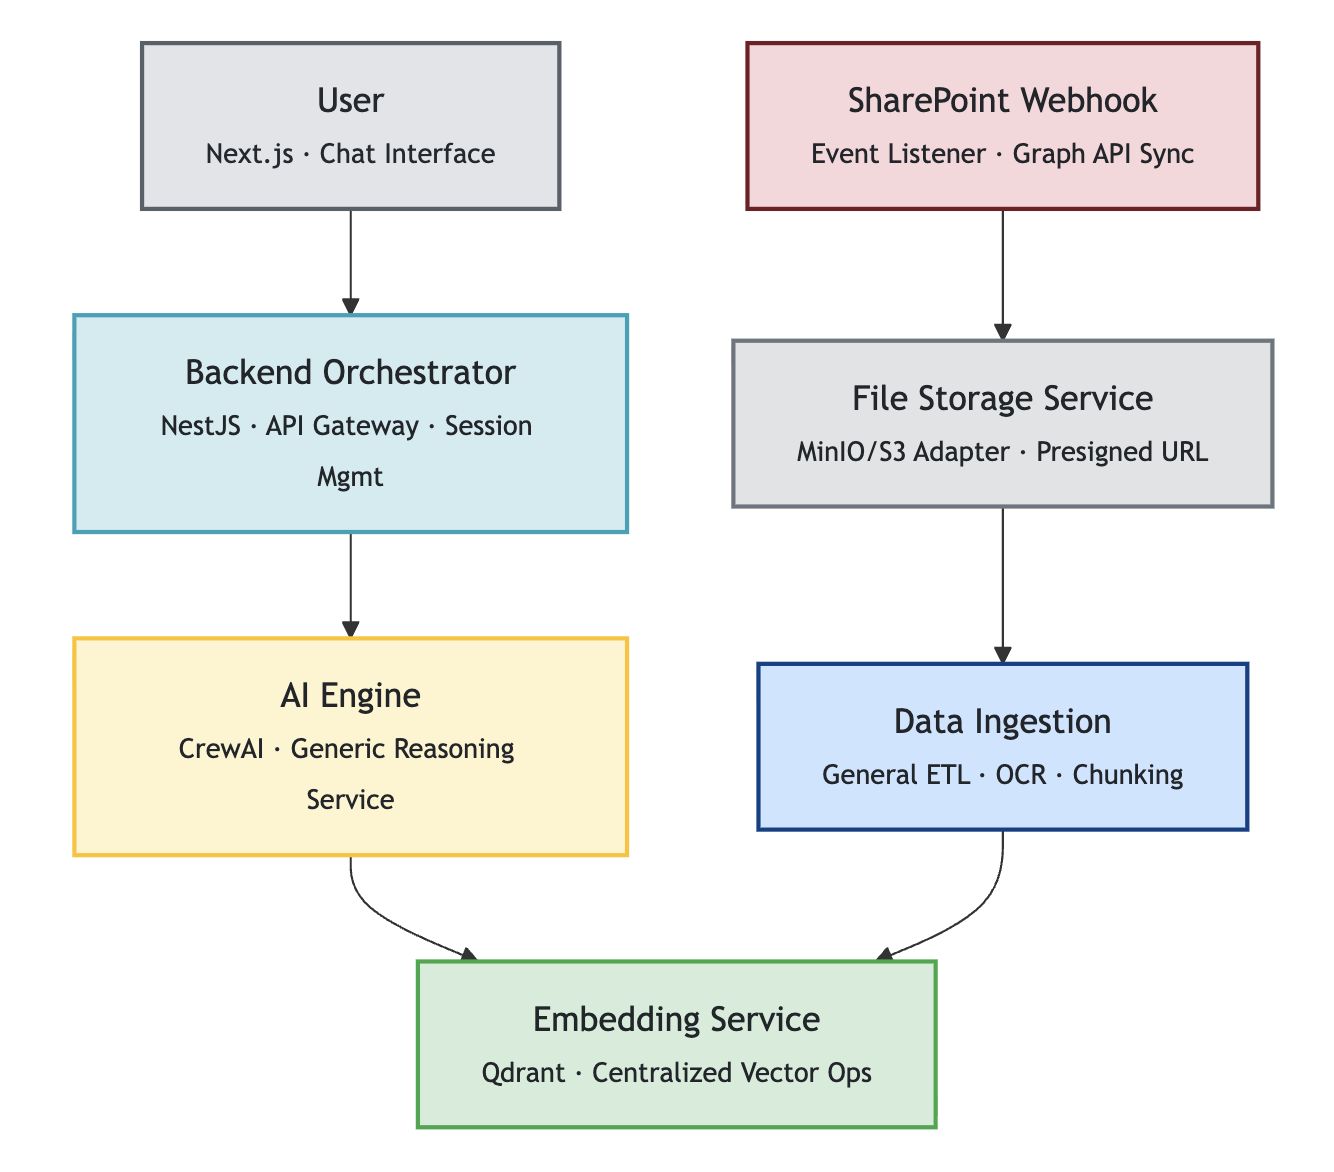
\includegraphics[width=5.35271in,height=4.68514in]{media/media/image6.png}

\textbf{Fig 1.} C4 Level 2 Diagram of the AiQ System

\textbf{Workflows}

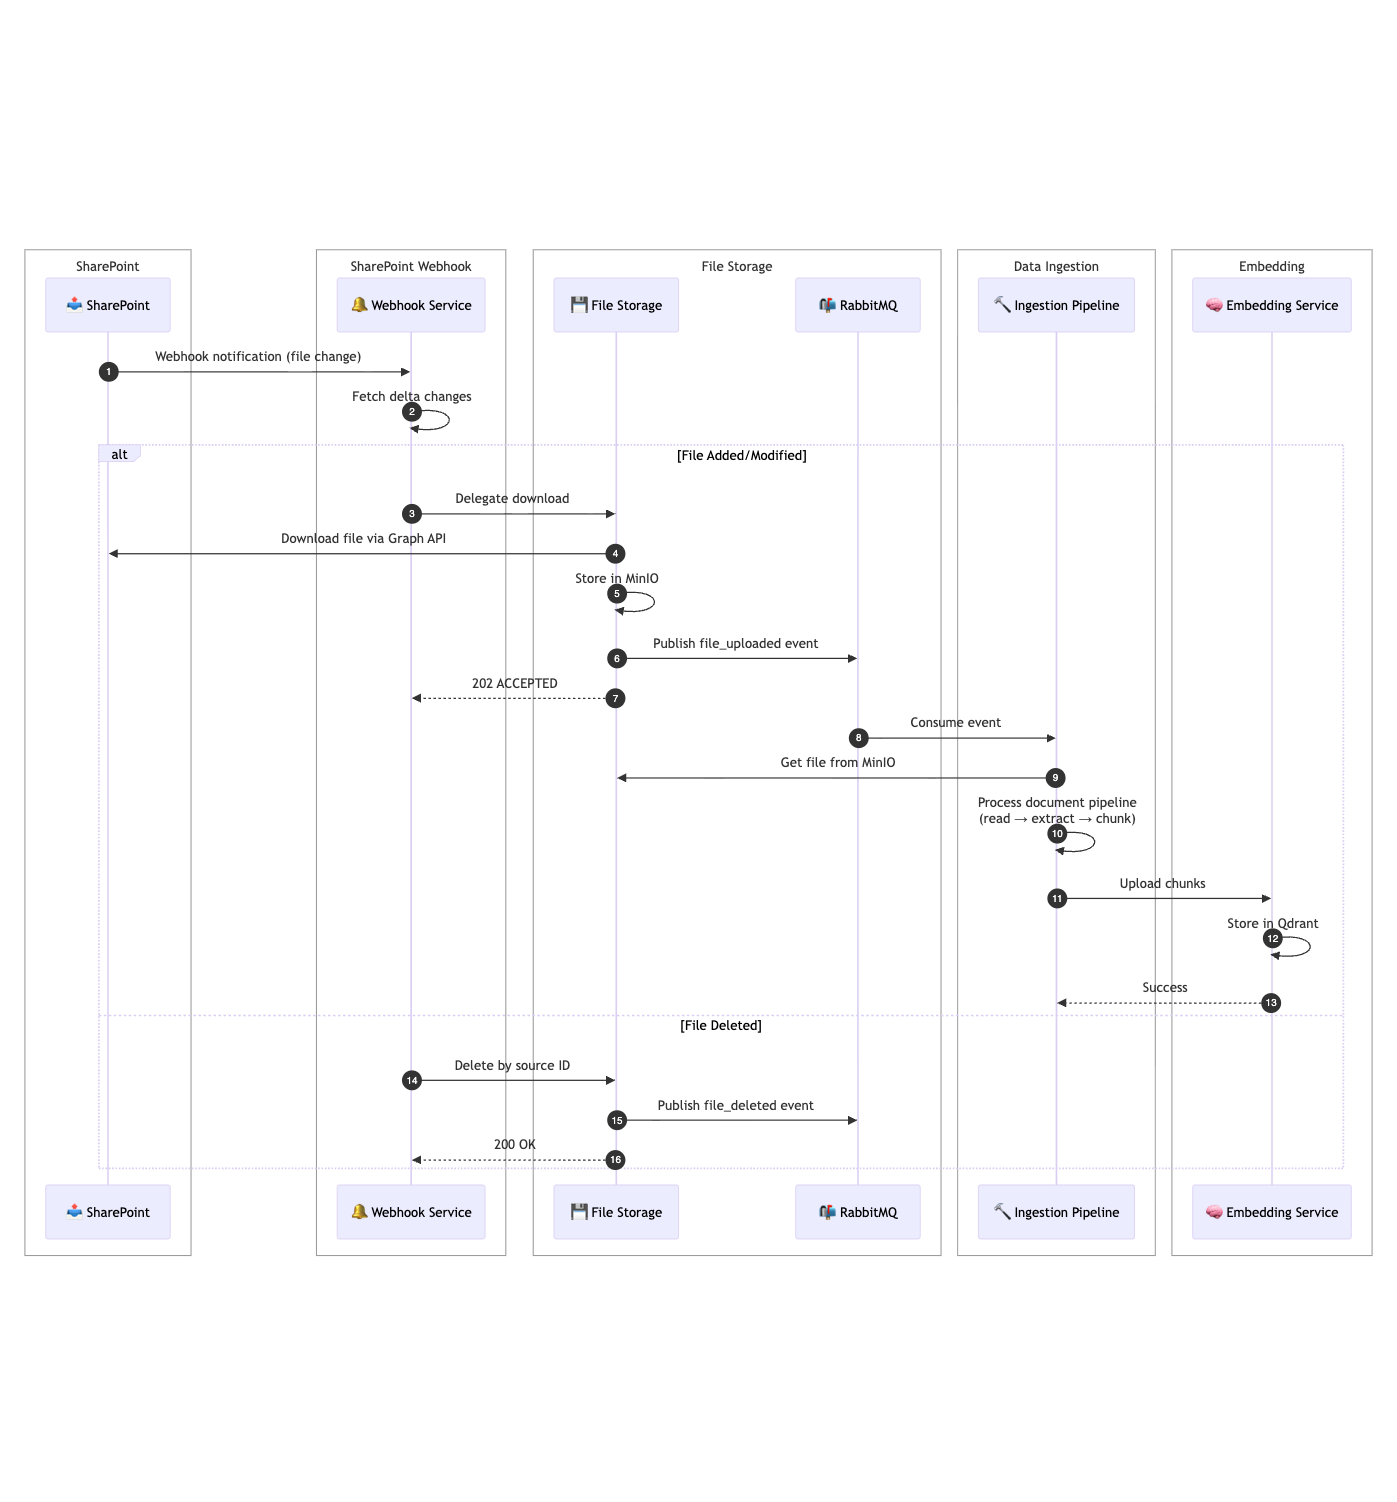
\includegraphics[width=6.26772in,height=4.72222in]{media/media/image5.png}

\textbf{Fic 2.} Sequence Diagram of RAG \& Agentic

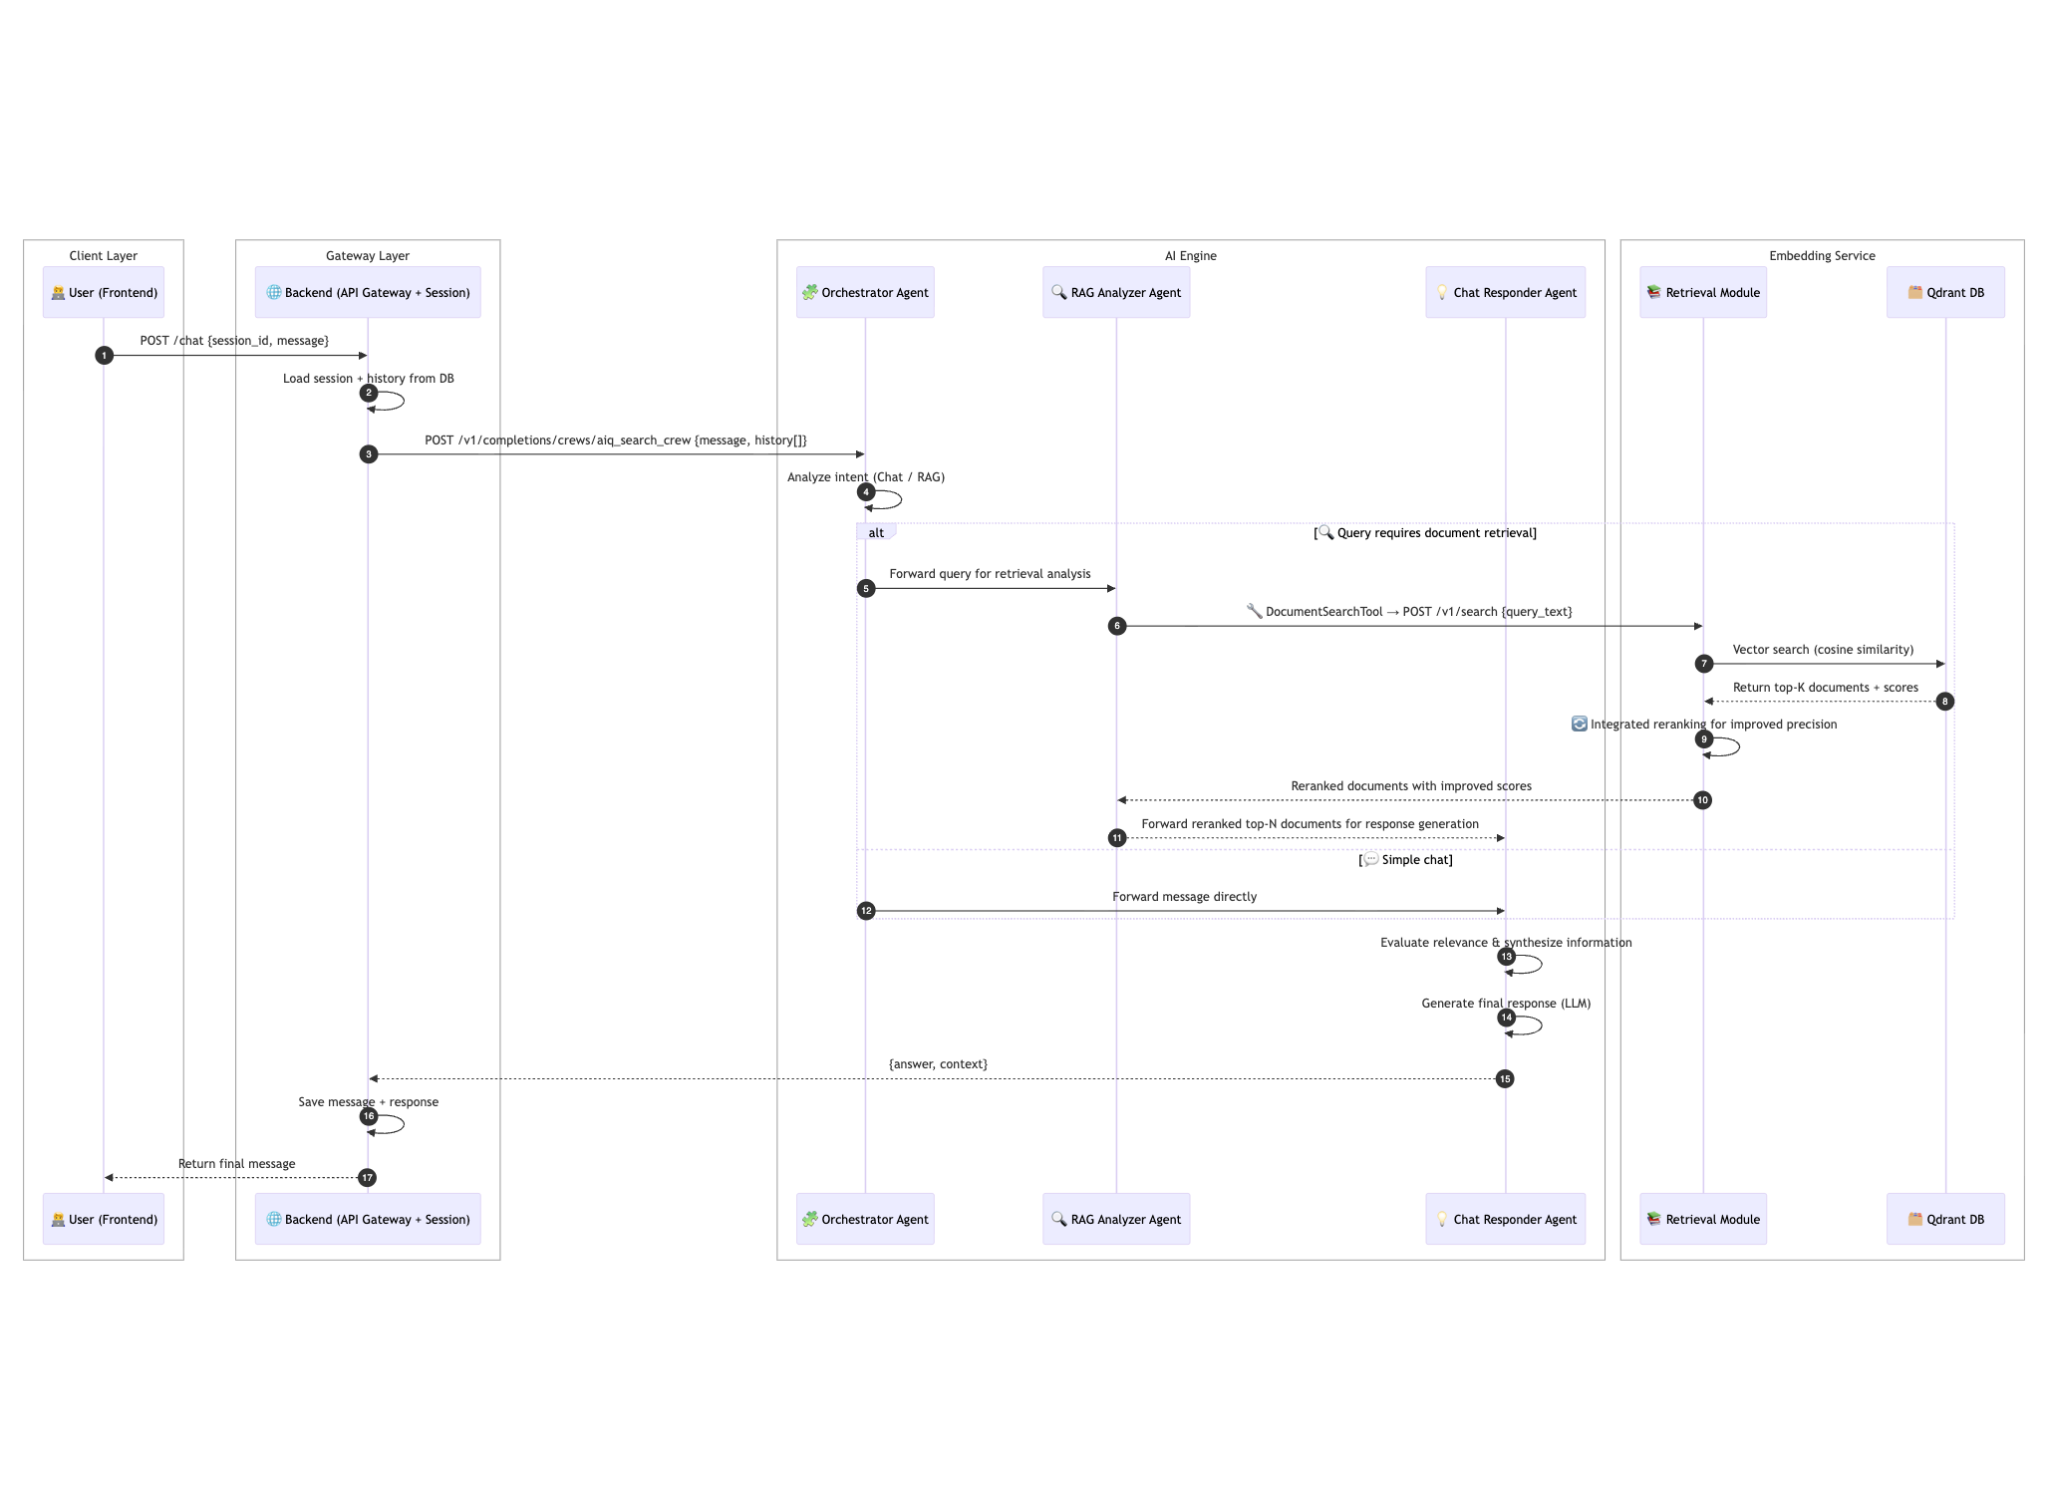
\includegraphics[width=6.26772in,height=3.41667in]{media/media/image4.png}

\textbf{Fig 3.} Sequence Diagram of the Data Ingestion Pipeline

\section{4. Teamwork Plan}\label{teamwork-plan}

\subsection{4.1 Roles and
Responsibilities}\label{roles-and-responsibilities}

\begin{enumerate}
\def\labelenumi{\arabic{enumi}.}
\item
  \textbf{Data Engineer:} Designs and develops the data pipeline for
  extracting and transforming information from multiple document formats
  (PDF, DOCX, PPTX, images). Ensures data quality, proper storage in the
  database, and readiness for use in the RAG system.
\item
  \textbf{Project Manager:} Manage project structure and timeline,
  communication across team members, track progress, and ensure that all
  results meet objectives.
\item
  \textbf{Web Developer:} Develop a web application, including a
  document upload system, Chat UI, and integrations with backend APIs.
  Also designs UX/UI for the web.
\item
  \textbf{AI Engineer:} Responsible for designing and developing AI
  components such as AI Agents, the RAG system, retrieval pipelines, and
  pipeline optimization to ensure accurate, efficient, and reliable
  performance for the AiQ platform.
\end{enumerate}

\subsection{4.2 Collaborative Plan}\label{collaborative-plan}

Scrum approach with bi-weekly sprints, where tasks are clearly defined
and tracked through Jira. The team conducts stand-up meetings 2--3 times
per week to maintain visibility of progress and to identify and resolve
blockers early.

\subsection{4.3 Task Coverage}\label{task-coverage}

\begin{enumerate}
\def\labelenumi{\arabic{enumi}.}
\item
  \textbf{Data ingestion \& Processing:} Data Engineer
\item
  \textbf{AI Components:} AI Engineer
\item
  \textbf{Backend API \& Frontend Interface:} Fullstack Developer
\item
  \textbf{Coordination, Documentation, Stakeholder
  Communication:}Project Manager
\end{enumerate}

\subsection{4.4 Workload Balance}\label{workload-balance}

Work is distributed according to each member's specialty. Story points
are assigned to ensure tasks are fairly distributed across each sprint
(following Scrum principles), so that every team member receives an
appropriate amount of work.

\section{}\label{section-2}

\section{5. Timeline}\label{timeline}

\section{\texorpdfstring{ Semester 1}{ Semester 1}}\label{semester-1}

{\def\LTcaptype{none} % do not increment counter
\begin{longtable}[]{@{}
  >{\raggedright\arraybackslash}p{(\linewidth - 4\tabcolsep) * \real{0.1515}}
  >{\raggedright\arraybackslash}p{(\linewidth - 4\tabcolsep) * \real{0.4242}}
  >{\raggedright\arraybackslash}p{(\linewidth - 4\tabcolsep) * \real{0.4242}}@{}}
\toprule\noalign{}
\begin{minipage}[b]{\linewidth}\centering
\textbf{Week}
\end{minipage} & \begin{minipage}[b]{\linewidth}\centering
\textbf{Task / Milestone}
\end{minipage} & \begin{minipage}[b]{\linewidth}\centering
\textbf{Deliverable}
\end{minipage} \\
\begin{minipage}[b]{\linewidth}\centering
Week 1--2
\end{minipage} & \begin{minipage}[b]{\linewidth}\centering
Conduct literature review and study relevant background materials
\end{minipage} & \begin{minipage}[b]{\linewidth}\centering
Review related work and draft the background, problem statement, and
project scope
\end{minipage} \\
\begin{minipage}[b]{\linewidth}\centering
Week 3--4
\end{minipage} & \begin{minipage}[b]{\linewidth}\centering
Gather requirements from users and stakeholders
\end{minipage} & \begin{minipage}[b]{\linewidth}\centering
Define project objectives, and write epics, user stories, and acceptance
criteria
\end{minipage} \\
\begin{minipage}[b]{\linewidth}\centering
Week 5--7
\end{minipage} & \begin{minipage}[b]{\linewidth}\centering
System-level architecture design, tool selection, model selection, and
data flow design
\end{minipage} & \begin{minipage}[b]{\linewidth}\centering
Draft architecture diagram, technology/tool stack list, model selection
justification
\end{minipage} \\
\begin{minipage}[b]{\linewidth}\centering
Week 8--10
\end{minipage} & \begin{minipage}[b]{\linewidth}\centering
Develop end-to-end web application (UI, backend APIs, database) without
data ingestion service
\end{minipage} & \begin{minipage}[b]{\linewidth}\centering
Functional prototype of the web application \& API documentation
\end{minipage} \\
\begin{minipage}[b]{\linewidth}\centering
Week 11--12
\end{minipage} & \begin{minipage}[b]{\linewidth}\centering
Investigate, design, and prototype Data Ingestion Service (pipeline,
ETL/ELT approach, orchestration)
\end{minipage} & \begin{minipage}[b]{\linewidth}\centering
Data ingestion service prototype \& ingestion workflow diagram
\end{minipage} \\
\begin{minipage}[b]{\linewidth}\centering
Week 13--14
\end{minipage} & \begin{minipage}[b]{\linewidth}\centering
Integrate and build end-to-end Data Ingestion Service with the existing
web application
\end{minipage} & \begin{minipage}[b]{\linewidth}\centering
Fully integrated data ingestion pipeline \& system integration test
report
\end{minipage} \\
\begin{minipage}[b]{\linewidth}\centering
Week 15-16
\end{minipage} & \begin{minipage}[b]{\linewidth}\centering
Final proposal presentation, documentation, and refinement
\end{minipage} & \begin{minipage}[b]{\linewidth}\centering
Final report \& final slides
\end{minipage} \\
\midrule\noalign{}
\endhead
\bottomrule\noalign{}
\endlastfoot
\end{longtable}
}

\section{\texorpdfstring{ Semester 2}{ Semester 2}}\label{semester-2}

{\def\LTcaptype{none} % do not increment counter
\begin{longtable}[]{@{}
  >{\raggedright\arraybackslash}p{(\linewidth - 4\tabcolsep) * \real{0.1530}}
  >{\raggedright\arraybackslash}p{(\linewidth - 4\tabcolsep) * \real{0.4227}}
  >{\raggedright\arraybackslash}p{(\linewidth - 4\tabcolsep) * \real{0.4243}}@{}}
\toprule\noalign{}
\begin{minipage}[b]{\linewidth}\centering
\textbf{Week}
\end{minipage} & \begin{minipage}[b]{\linewidth}\centering
\textbf{Task / Milestone}
\end{minipage} & \begin{minipage}[b]{\linewidth}\centering
\textbf{Deliverable}
\end{minipage} \\
\begin{minipage}[b]{\linewidth}\centering
Week 1--2
\end{minipage} & \begin{minipage}[b]{\linewidth}\centering
Enhance ingestion pipeline, optimize chatbot performance, and run
initial evaluations
\end{minipage} & \begin{minipage}[b]{\linewidth}\centering
Updated ingestion pipeline, baseline performance metrics, initial
evaluation report
\end{minipage} \\
\begin{minipage}[b]{\linewidth}\centering
Week 3--4
\end{minipage} & \begin{minipage}[b]{\linewidth}\centering
Further optimization: ingestion improvements, better accuracy \& lower
latency, continued evaluations
\end{minipage} & \begin{minipage}[b]{\linewidth}\centering
Optimized ingestion v2, improved model performance metrics, mid-phase
progress report
\end{minipage} \\
\begin{minipage}[b]{\linewidth}\centering
Week 5--7
\end{minipage} & \begin{minipage}[b]{\linewidth}\centering
Build and refine key web features (citations, SSO, UI/UX improvements)
\end{minipage} & \begin{minipage}[b]{\linewidth}\centering
Completed core web functionality, demo-ready feature build
\end{minipage} \\
\begin{minipage}[b]{\linewidth}\centering
Week 8--10
\end{minipage} & \begin{minipage}[b]{\linewidth}\centering
Product polishing: bug fixing, refinement, readiness for User Acceptance
Testing (UAT)
\end{minipage} & \begin{minipage}[b]{\linewidth}\centering
Pre-UAT build, UAT checklist \& test cases
\end{minipage} \\
\begin{minipage}[b]{\linewidth}\centering
Week 11--12
\end{minipage} & \begin{minipage}[b]{\linewidth}\centering
Conduct UAT and begin final report
\end{minipage} & \begin{minipage}[b]{\linewidth}\centering
UAT results, defect list, draft final report
\end{minipage} \\
\begin{minipage}[b]{\linewidth}\centering
Week 13--14
\end{minipage} & \begin{minipage}[b]{\linewidth}\centering
Resolve UAT issues, performance stabilization
\end{minipage} & \begin{minipage}[b]{\linewidth}\centering
Resolved issue log, final system build
\end{minipage} \\
\begin{minipage}[b]{\linewidth}\centering
Week 15-16
\end{minipage} & \begin{minipage}[b]{\linewidth}\centering
Deliver final report and presentation
\end{minipage} & \begin{minipage}[b]{\linewidth}\centering
Final written report, presentation slide deck, final demo
\end{minipage} \\
\midrule\noalign{}
\endhead
\bottomrule\noalign{}
\endlastfoot
\end{longtable}
}

\section{\texorpdfstring{6. Ethics, Privacy, and Professional
Considerations
}{6. Ethics, Privacy, and Professional Considerations }}\label{ethics-privacy-and-professional-considerations}

\subsubsection{\texorpdfstring{\textbf{6.1 Credibility of
Information}}{6.1 Credibility of Information}}\label{credibility-of-information}

Our project establishes data credibility by grounding all work in
dependable and well-validated materials. Internal documents from SCB
TechX provide accurate domain knowledge that reflects real workflows and
requirements. External information such as academic papers and official
documentation for tools and frameworks are carefully selected from
reliable sources. Together, these materials form a solid and reliable
knowledge base for the project.

\textbf{6.2 Intellectual Property \& Law}

All activities under this project adhere to confidentiality obligations
as defined in the Capstone Non-Disclosure Agreement (NDA) between SCB
Tech X and participating students. All proprietary information including
technical data, business information, processes, software, and internal
documentation remains the exclusive property of SCB Tech X and must not
be disclosed, reproduced, or used beyond the scope of the Capstone
project. Students must store confidential data securely, restrict access
only to authorized project members.

\section{References}\label{references}

{[}1{]} G. W. Furnas, T. K. Landauer, L. M. Gomez, and S. T. Dumais,
"The vocabulary problem in human-system communication," \emph{Commun.
ACM}, vol. 30, no. 11, pp. 964--971, Nov. 1987.

{[}2{]} P. Lewis \emph{et al.}, "Retrieval-Augmented Generation for
Knowledge-Intensive NLP Tasks," \emph{arXiv.org}, Apr. 12, 2021.
\href{https://arxiv.org/abs/2005.11401}{\ul{https://arxiv.org/abs/2005.11401}}

{[}3{]} S. Barnett, S. Kurniawan, S. Thudumu, Z. Brannelly, and M.
Abdelrazek, "Seven Failure Points When Engineering a Retrieval Augmented
Generation System," \emph{arXiv (Cornell University)}, Jan. 2024.
\href{https://arxiv.org/abs/2401.05856}{\ul{https://arxiv.org/abs/2401.05856}}

{[}4{]} D. Edge \emph{et al.}, "From Local to Global: A Graph RAG
Approach to Query-Focused Summarization," \emph{arXiv.org}, Apr. 24,
2024.
\href{https://arxiv.org/abs/2404.16130}{\ul{https://arxiv.org/abs/2404.16130}}

{[}5{]} Y. Gao \emph{et al.}, "Retrieval-Augmented Generation for Large
Language Models: A Survey," \emph{arXiv.org}, Dec. 18, 2023.
\href{https://arxiv.org/abs/2312.10997}{\ul{https://arxiv.org/abs/2312.10997}}

{[}6{]} Deep Search Team, ``Docling Technical Report,'' arXiv.org, Aug.
2024.
\href{https://arxiv.org/abs/2408.09869}{\ul{https://arxiv.org/abs/2408.09869}}

\section{\texorpdfstring{\hfill\break
}{ }}\label{section-3}

\section{Appendices}\label{appendices}

\subsection{Wireframes and Mockups}\label{wireframes-and-mockups}

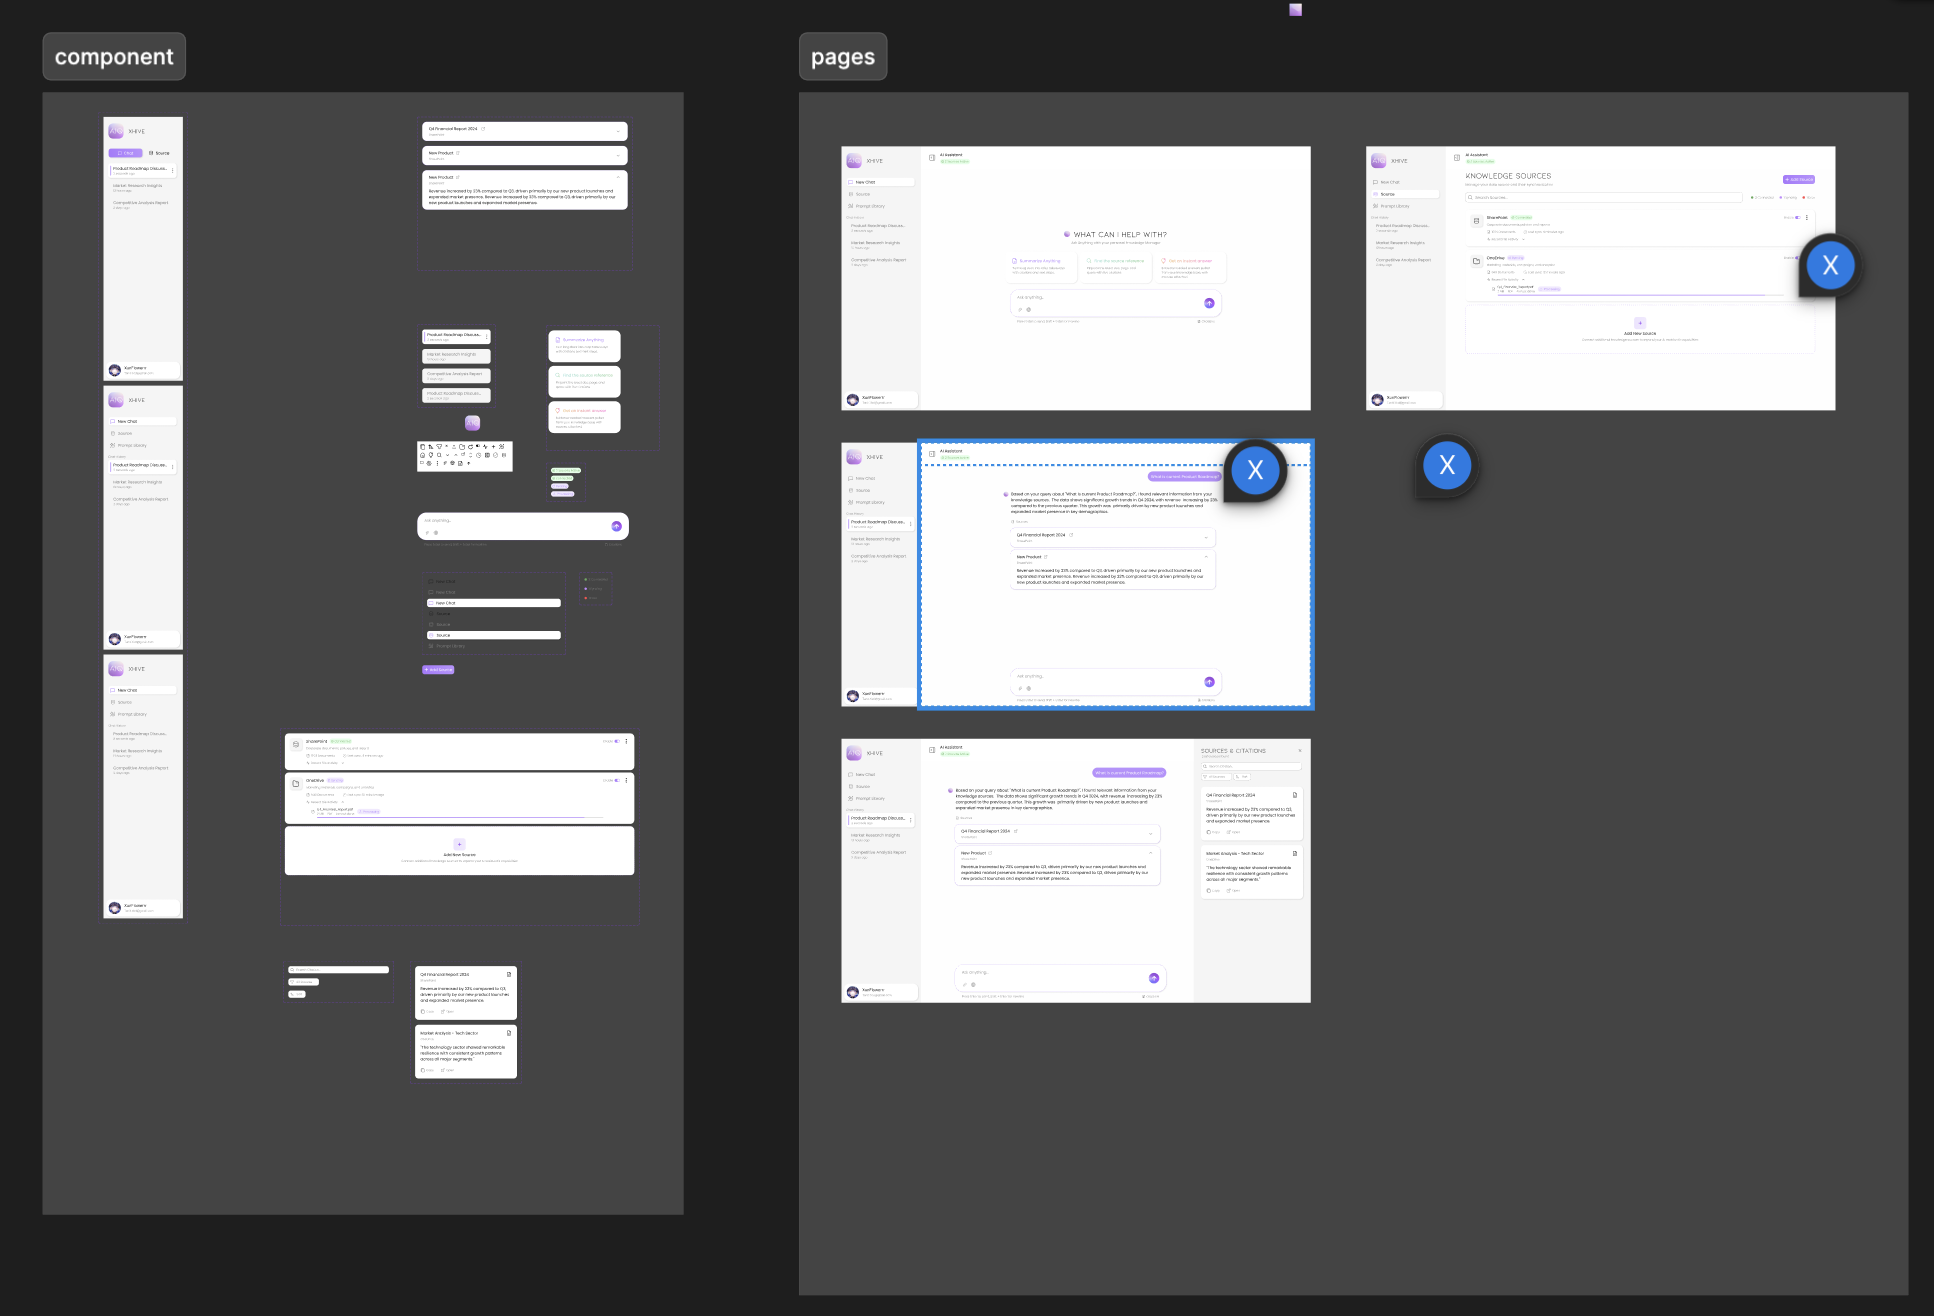
\includegraphics[width=6.26772in,height=4.26389in]{media/media/image7.png}

Figure 1: Figma components as our design system

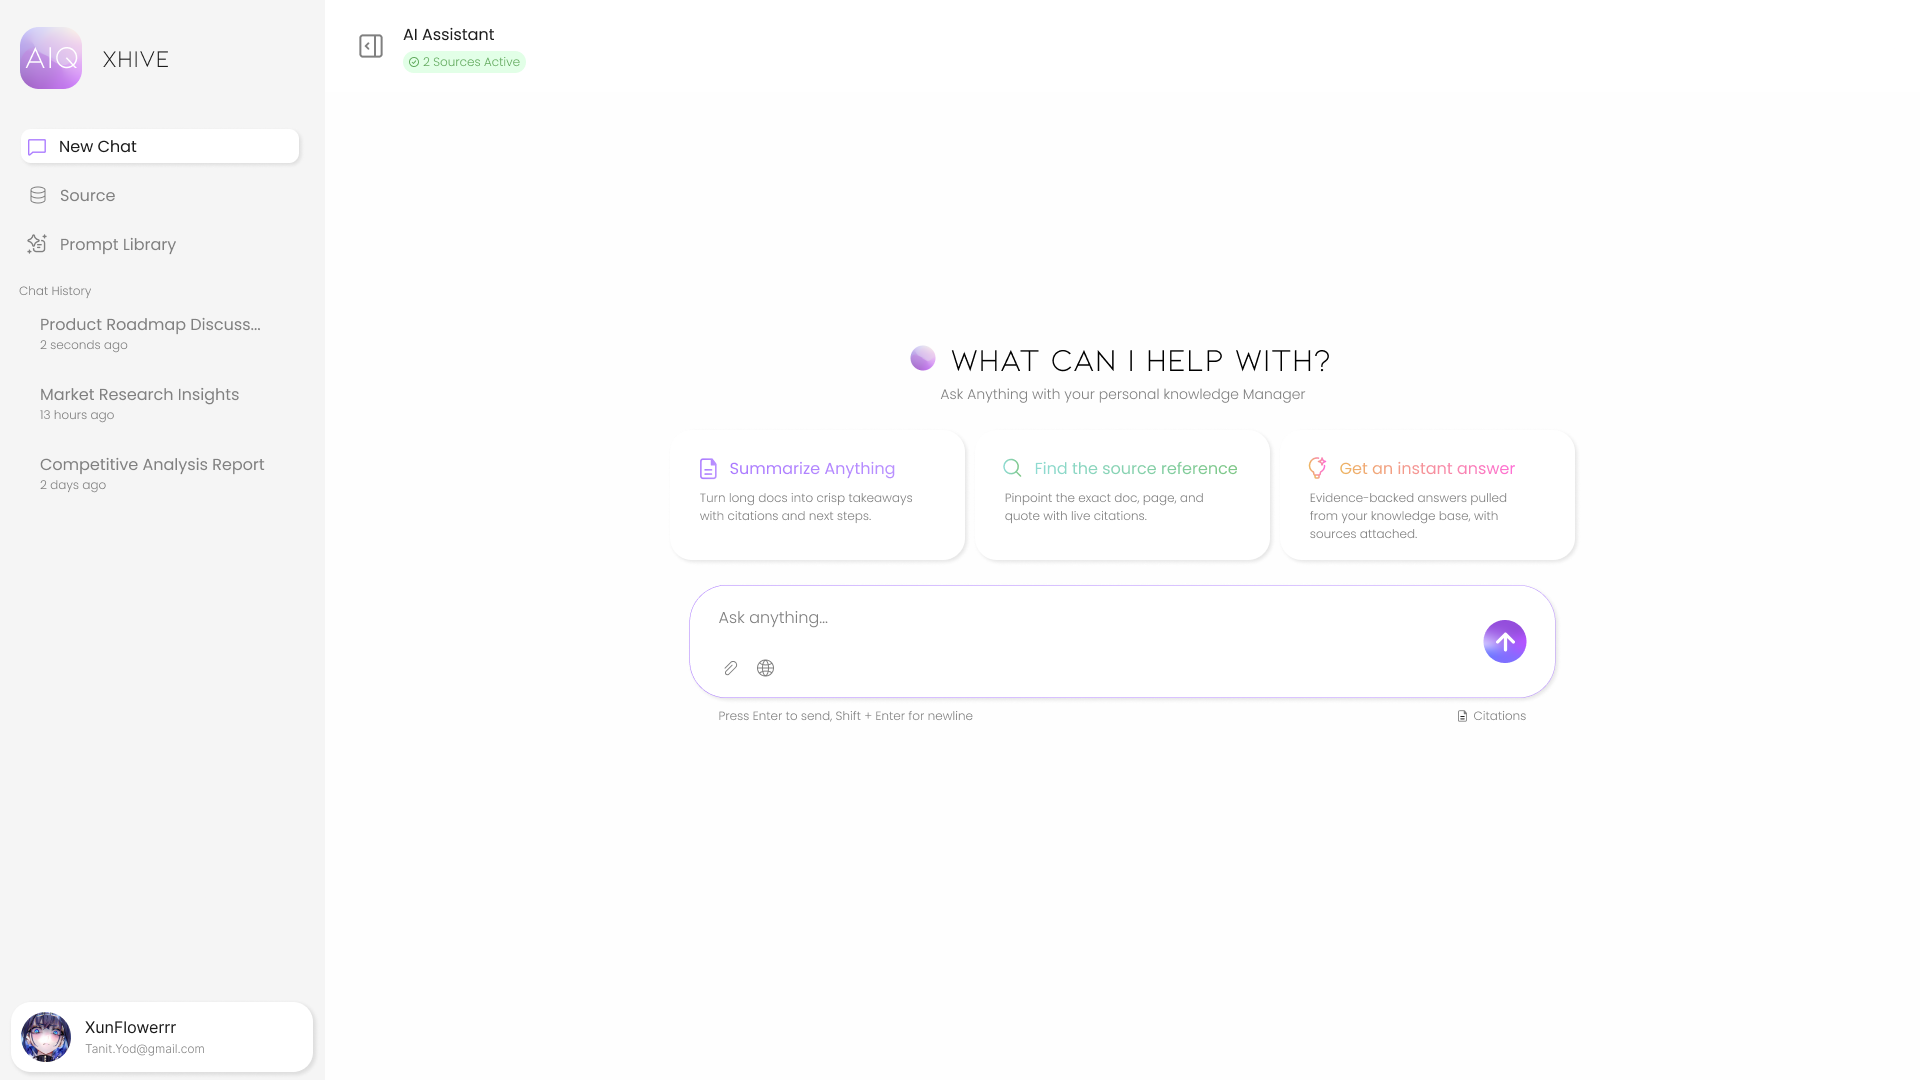
\includegraphics[width=6.26772in,height=3.52778in]{media/media/image2.png}

Figure 2: Web chat interface for demonstrating system intelligence

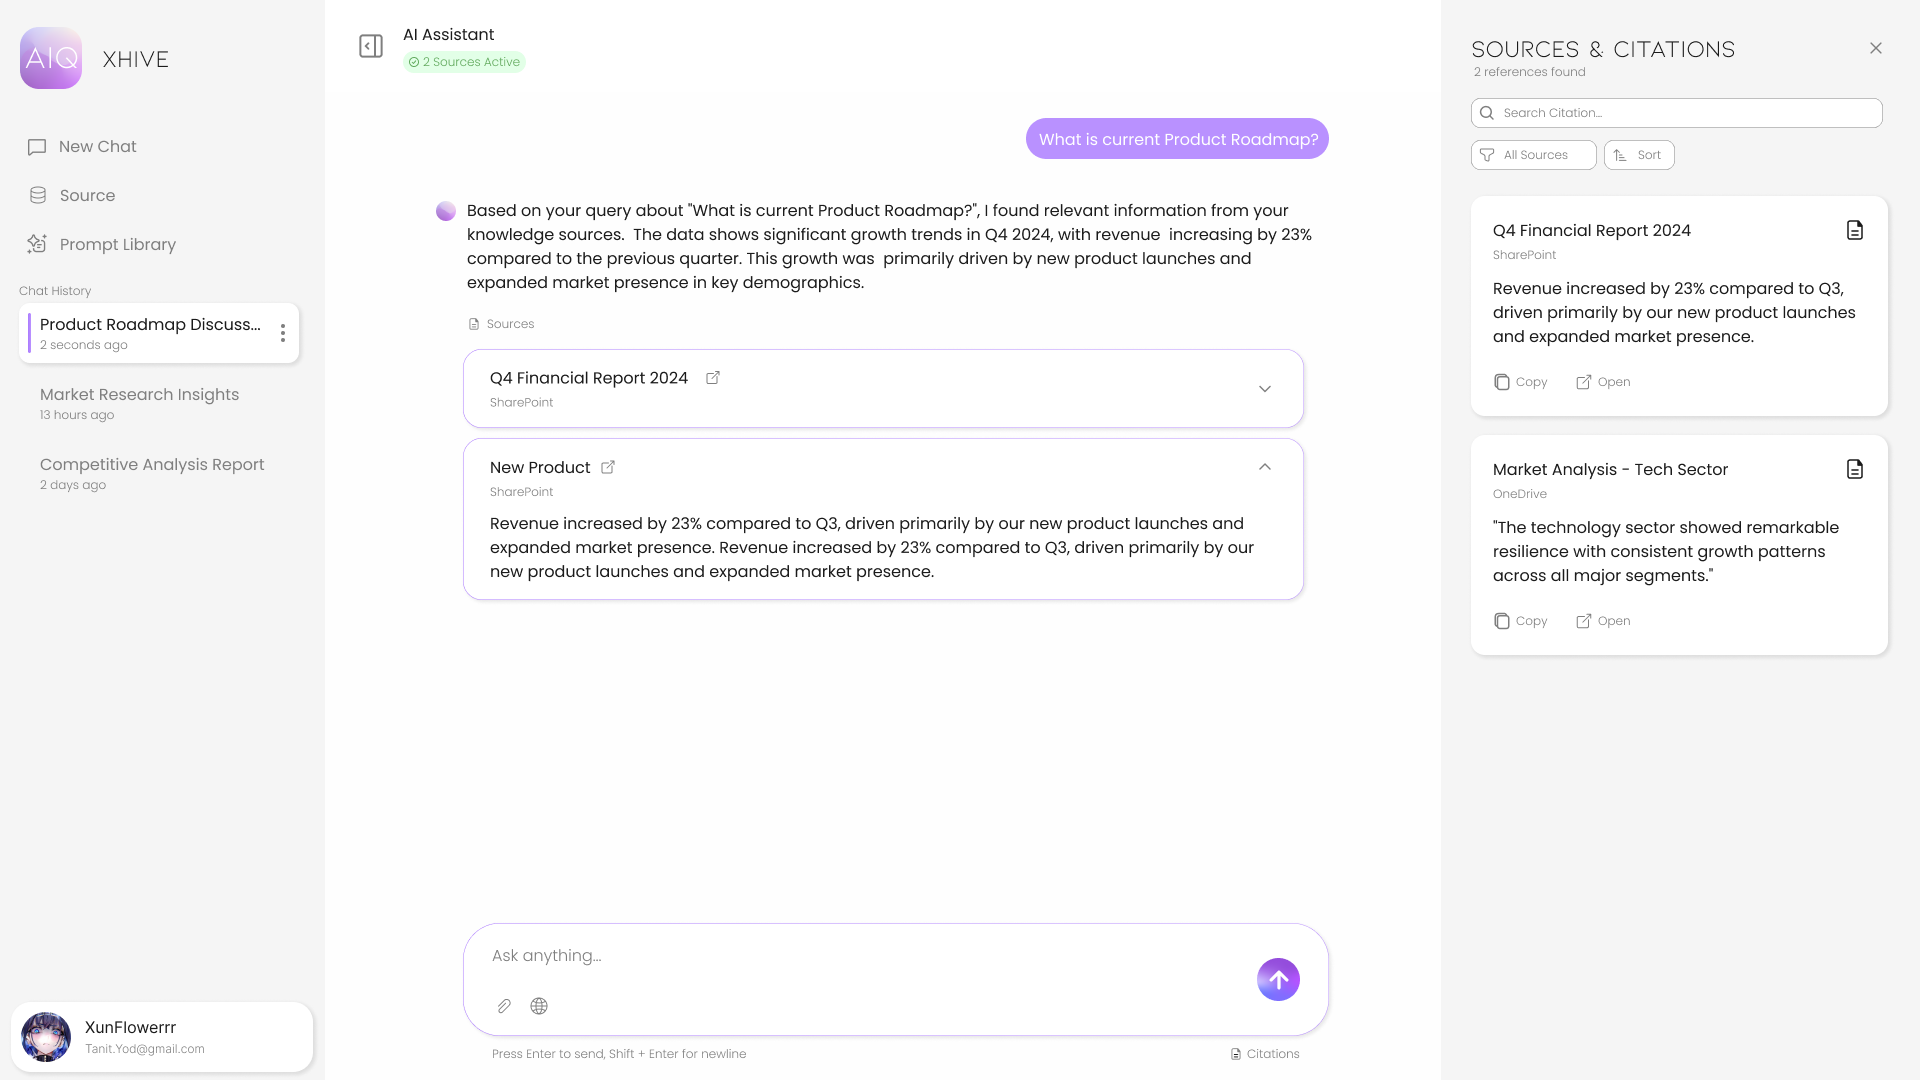
\includegraphics[width=6.26772in,height=3.52778in]{media/media/image1.png}

Figure 3: Web chat interface for viewing citation details

\subsection{Early Test Datasets}\label{early-test-datasets}

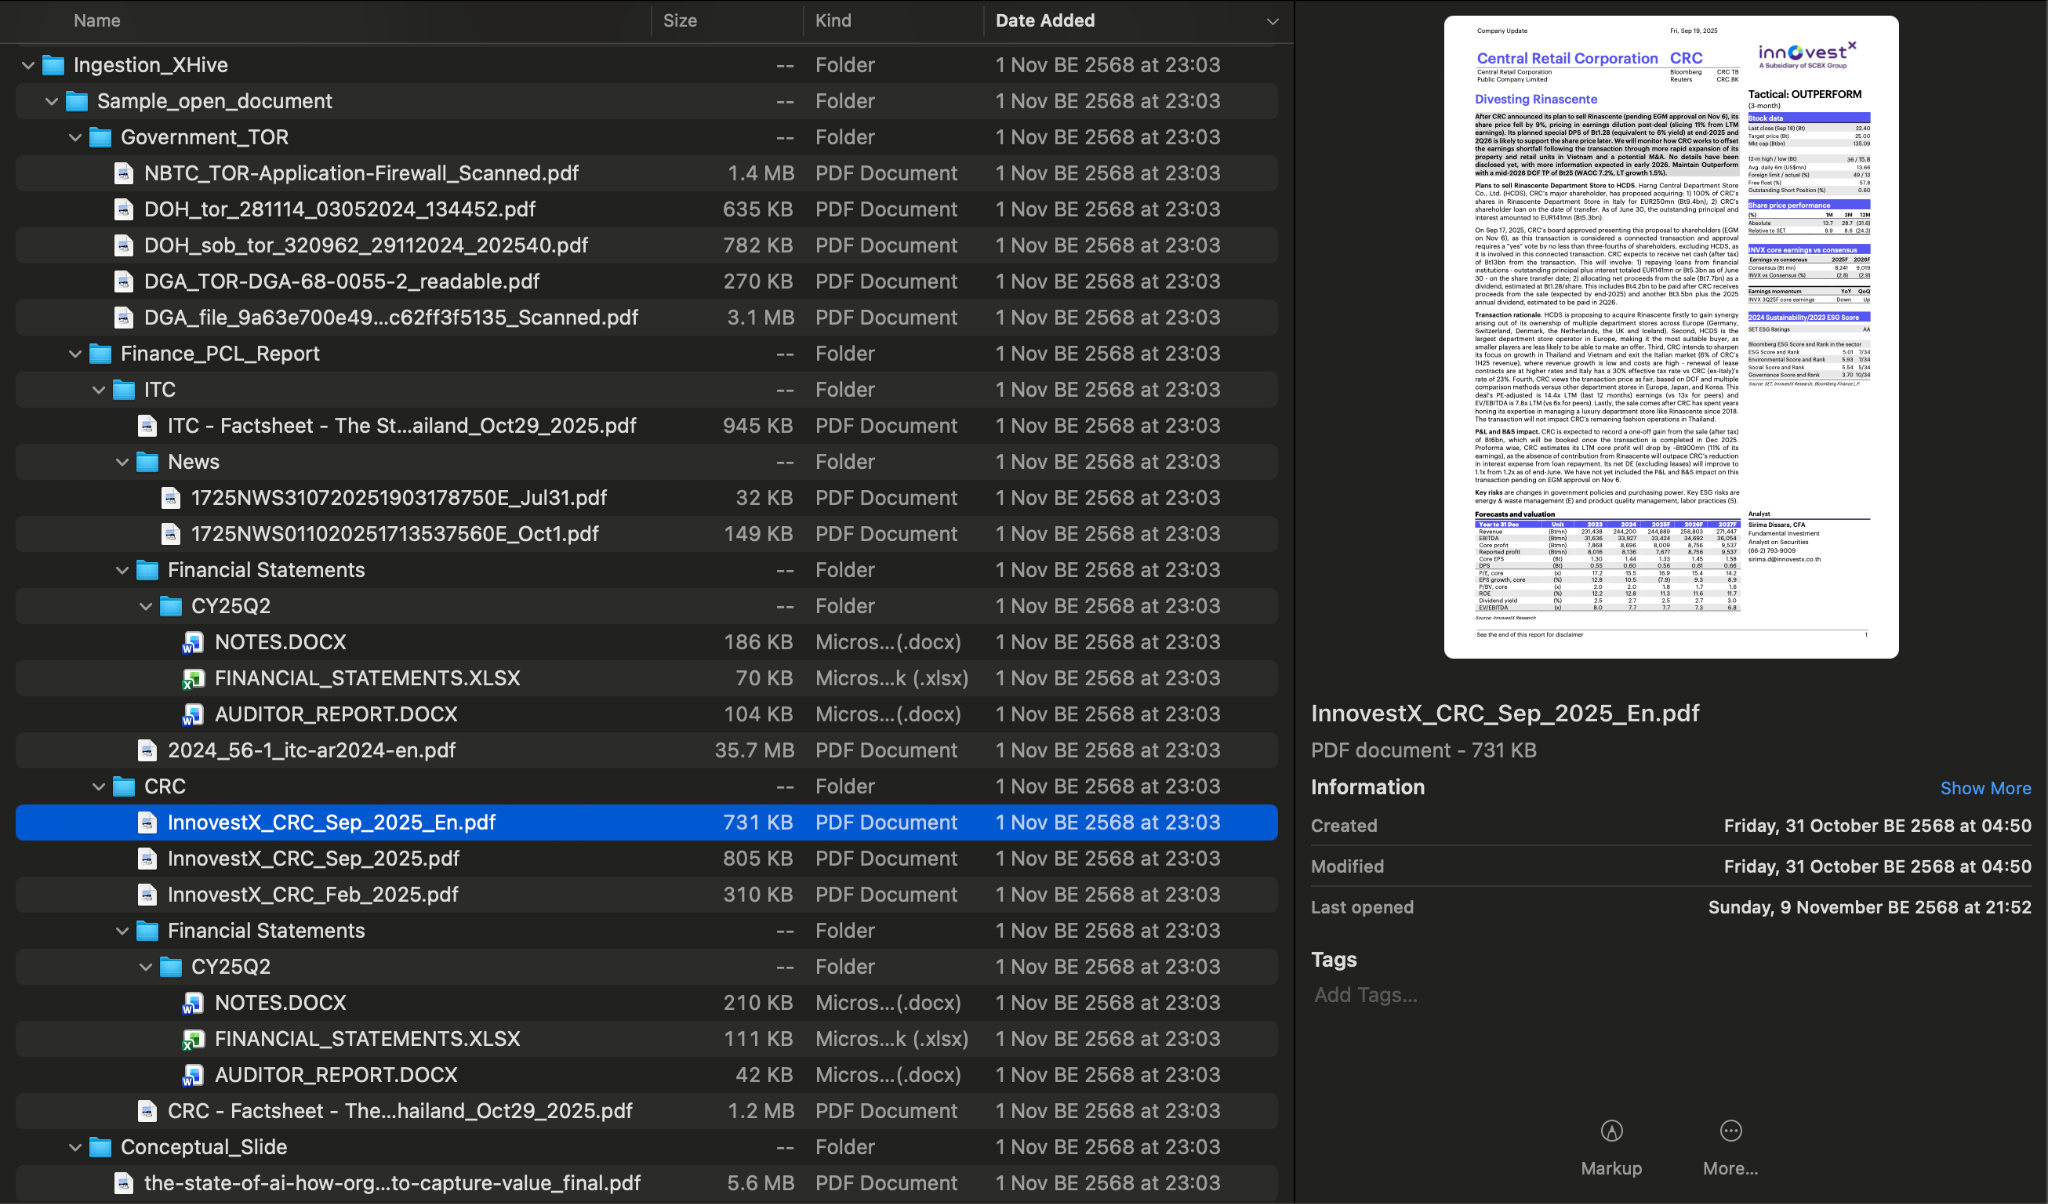
\includegraphics[width=6.26772in,height=3.68056in]{media/media/image3.png}

Figure 1: Example of test dataset
\end{document}
